\documentclass[tikz,border=12pt]{standalone}
% Estilo comum dos esquemas vetoriais das aulas da GA033.
\usepackage[T1]{fontenc}
\usepackage[utf8]{inputenc}
\usepackage{lmodern}
\usepackage{amsmath,amssymb}
\usetikzlibrary{arrows.meta,positioning,calc,fit,matrix,decorations.pathreplacing,backgrounds,shapes.geometric}
\definecolor{lnccblue}{HTML}{075AC0}
\definecolor{ink}{HTML}{242A31}
\definecolor{muted}{HTML}{647080}
\definecolor{lightblue}{HTML}{EFF5FC}
\definecolor{teal}{HTML}{197C83}
\definecolor{orange}{HTML}{BC6A16}
\tikzset{
  every node/.style={font=\sffamily\fontsize{15}{18}\selectfont,text=ink},
  box/.style={draw=lnccblue,line width=0.9pt,fill=lightblue,inner sep=9pt,align=center},
  flow/.style={-{Stealth[length=3mm,width=2mm]},draw=lnccblue,line width=1pt},
  point/.style={circle,draw=lnccblue,fill=white,line width=1.2pt,minimum size=3.2mm,inner sep=0pt},
  label/.style={font=\sffamily\fontsize{13}{16}\selectfont,text=muted},
  heading/.style={font=\sffamily\bfseries\fontsize{16}{19}\selectfont,text=lnccblue}
}
% Impede setas horizontais involuntariamente invertidas após editar os nós.
\newdimen\origemseta
\newdimen\destinoseta
\newcommand{\verificarsetadireita}[2]{%
  \pgfextractx{\origemseta}{\pgfpointanchor{#1}{east}}%
  \pgfextractx{\destinoseta}{\pgfpointanchor{#2}{west}}%
  \advance\origemseta by 4mm%
  \ifdim\destinoseta>\origemseta\else
    \PackageError{diagramas}{Conector sem espaco entre #1 e #2}{Afaste os nos antes de compilar.}%
  \fi
}

\begin{document}
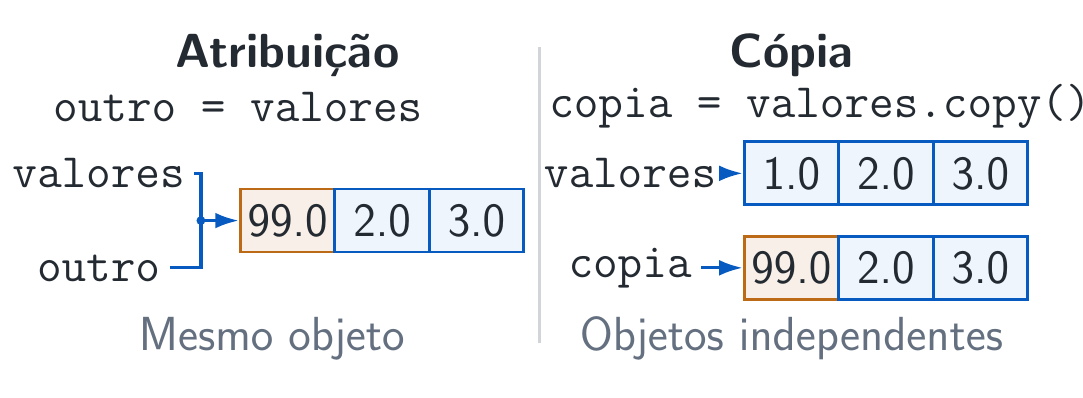
\begin{tikzpicture}[
  x=1cm,y=1cm,every node/.append style={font=\sffamily\fontsize{16}{20}\selectfont},
  seta/.style={-{Latex[length=3mm,width=2mm]},draw=lnccblue,line width=1.2pt},
  celula/.style={draw=lnccblue,line width=1pt,fill=lightblue,
    minimum width=1.2cm,minimum height=.8cm,inner sep=2pt}
]
\path[use as bounding box] (-.1,-2.35) rectangle (12.95,2.0);
\draw[draw=muted!30,line width=.8pt] (6.4,-2.0) -- (6.4,1.75);
\node[text=ink,font=\sffamily\fontsize{18}{22}\selectfont\bfseries] at (3.2,1.65) {Atribuição};
\node[text=ink,font=\sffamily\fontsize{18}{22}\selectfont\bfseries] at (9.6,1.65) {Cópia};
\node[anchor=west,text=ink] at (.1,1.0) {\texttt{outro = valores}};
\node[anchor=west,text=ink] at (6.4,1.0) {\texttt{copia = valores.copy()}};

\node[text=ink] (nome1) at (.8,.15) {\texttt{valores}};
\node[text=ink] (nome2) at (.8,-1.05) {\texttt{outro}};
\node[celula,fill=orange!10,draw=orange] (a0) at (3.2,-.45) {99.0};
\node[celula] at (4.4,-.45) {2.0};
\node[celula] at (5.6,-.45) {3.0};
\coordinate (compartilhado) at (2.1,-.45);
\draw[lnccblue,line width=1.2pt] (nome1.east) -| (compartilhado);
\draw[lnccblue,line width=1.2pt] (nome2.east) -| (compartilhado);
\fill[lnccblue] (compartilhado) circle[radius=1.6pt];
\verificarsetadireita{compartilhado}{a0}
\draw[seta] (compartilhado) -- (a0.west);
\node[text=muted,align=center] at (3.0,-1.95) {Mesmo objeto};

\node[text=ink] (original) at (7.55,.15) {\texttt{valores}};
\node[text=ink] (copia) at (7.55,-1.05) {\texttt{copia}};
\node[celula] (o0) at (9.6,.15) {1.0};
\node[celula] at (10.8,.15) {2.0};
\node[celula] at (12.0,.15) {3.0};
\node[celula,fill=orange!10,draw=orange] (c0) at (9.6,-1.05) {99.0};
\node[celula] at (10.8,-1.05) {2.0};
\node[celula] at (12.0,-1.05) {3.0};
\draw[seta] (original.east) -- (o0.west);
\draw[seta] (copia.east) -- (c0.west);
\node[text=muted,align=center] at (9.6,-1.95) {Objetos independentes};
\end{tikzpicture}
\end{document}
